%%%%%%%%%%%%%%%%%%%%%%%%%%%%%%%%%%%%%%%%%%%%%%%%%%%%%%%%%%%%%%%%%%%%%%%%
%% Project 9: ML for SIEM Alert Triage
%% Student: Yogita
%% Format: IEEE Conference (IEEEtran)
%%%%%%%%%%%%%%%%%%%%%%%%%%%%%%%%%%%%%%%%%%%%%%%%%%%%%%%%%%%%%%%%%%%%%%%%
\documentclass[conference]{IEEEtran}

% ---- Packages ----
\usepackage[utf8]{inputenc}
\usepackage[T1]{fontenc}
\usepackage{amsmath,amssymb}
\usepackage{graphicx}
\usepackage{booktabs}
\usepackage{hyperref}
\usepackage{cite}
\usepackage{xcolor}
\usepackage{algorithm}
\usepackage{algorithmic}
\usepackage{multirow}
\usepackage{balance}

\hypersetup{
  colorlinks=true,
  linkcolor=blue,
  citecolor=blue,
  urlcolor=blue,
}

% Path to figures
\graphicspath{{../outputs/}}

\begin{document}

% ---- Title ----
\title{Cost-Sensitive Ensemble Machine Learning\\for SIEM Alert Triage: Reducing Alert Fatigue\\Through Stacking Classification}

\author{
  \IEEEauthorblockN{Yogita}
  \IEEEauthorblockA{
    Department of AI/ML\\
    \textit{Graduate Research Project}\\
  }
}

\maketitle

% ---- Abstract ----
\begin{abstract}
Security Information and Event Management (SIEM) systems generate an overwhelming volume of alerts, the vast majority of which are false positives.
This alert fatigue leads analysts to miss genuine threats and degrades the effectiveness of Security Operations Centers (SOCs).
We propose a cost-sensitive stacking ensemble that combines Random Forest, XGBoost, and Isolation Forest anomaly scores with a Logistic Regression meta-learner to perform three-class alert triage: True Positive, False Positive, and Indeterminate.
Our cost function penalises missed true positives (false negatives) at $10\times$ the cost of false positive escalations, directly encoding the asymmetric risk of security operations.
Evaluated on synthetic datasets modelled after CIC-IDS2017, NSL-KDD, and UNSW-NB15, the stacking ensemble achieves strong $F_{\beta=2}$ scores while significantly reducing alert volume.
SHAP-based explanations identify the most influential alert features, providing interpretable decision support for analysts.
The system demonstrates that intelligent ML-driven triage can substantially reduce analyst workload without compromising threat detection.
\end{abstract}

\begin{IEEEkeywords}
SIEM, alert triage, cost-sensitive learning, ensemble methods, stacking classifier, alert fatigue, XGBoost, Random Forest, Isolation Forest, SHAP
\end{IEEEkeywords}

% ==================================================================
\section{Introduction}
\label{sec:introduction}

Modern enterprises rely on Security Information and Event Management (SIEM) systems to aggregate and correlate security events from firewalls, intrusion detection systems (IDS), endpoints, and cloud infrastructure~\cite{tariq2025}.
However, the volume of alerts generated daily---often tens of thousands---far exceeds the capacity of human analysts, with false positive rates commonly reported above 80\%~\cite{khayat2025, ghadermazi2024}.
This phenomenon, widely known as \emph{alert fatigue}, causes analysts to overlook genuine threats, increases mean time to respond (MTTR), and contributes to analyst burnout~\cite{ban2023}.

Recent work has explored machine learning approaches to alert triage, including graph-based prioritisation~\cite{malach2025}, context-aware alert prioritisation~\cite{wang2024}, and empirical measurement of alert accuracy in production SOCs~\cite{yang2024}.
While promising, many existing methods treat the problem as binary classification (benign vs.\ malicious) and fail to account for the \emph{asymmetric costs} inherent in security operations: missing a true attack is far more damaging than investigating a false alarm~\cite{srinivas2025}.

In this work, we address these limitations through three contributions:

\begin{enumerate}
  \item \textbf{Three-class triage}: We formulate alert triage as a three-class problem (True Positive, False Positive, Indeterminate), reflecting real-world SOC workflows where uncertain alerts require additional investigation rather than outright dismissal.
  \item \textbf{Cost-sensitive stacking ensemble}: We combine Random Forest with class-weighted losses, XGBoost with sample-level cost weights, and Isolation Forest anomaly scores within a stacking architecture.  The meta-learner (Logistic Regression) fuses predictions to maximise $F_{\beta=2}$, which prioritises recall to minimise missed threats.
  \item \textbf{Explainable triage}: We apply SHAP (SHapley Additive exPlanations) to identify the features most influential in classifying an alert as a true positive, providing actionable insight for analysts.
\end{enumerate}

% ==================================================================
\section{Related Work}
\label{sec:related}

\subsection{Alert Triage in SOCs}
Ban et al.~\cite{ban2023} proposed an AI-assisted SIEM framework for breaking alert fatigue through effective incident response using random forests and gradient boosting.
Ghadermazi et al.~\cite{ghadermazi2024} developed a machine learning and optimisation framework for efficient alert management in cybersecurity operations centres.
Khayat et al.~\cite{khayat2025} provided a systematic literature review on empowering SOCs with AI and ML, identifying ensemble methods and cost-sensitive learning as key research gaps.

\subsection{Cost-Sensitive and Ensemble Methods}
Malach et al.~\cite{malach2025} proposed CyberShapley, which uses informative graph representations for explanation, prioritisation, and triage of cybersecurity alerts.
Srinivas et al.~\cite{srinivas2025} surveyed AI-augmented SOC approaches using LLMs and agents for security automation, including ensemble strategies for alert fatigue reduction.

\subsection{Deep Learning and Advanced Approaches}
Wang et al.~\cite{wang2024} proposed AlertPro, a context-aware alert prioritisation system using reinforcement learning for multi-step attack detection.
Yang et al.~\cite{yang2024} presented an empirical measurement of network alerts in a SOC at USENIX Security 2024, distinguishing true attacks from benign triggers.
Tariq et al.~\cite{tariq2025} surveyed alert fatigue in security operations centres, highlighting research challenges and opportunities for cost-aware and explainable models.

% ==================================================================
\section{Methodology}
\label{sec:methodology}

\subsection{Problem Formulation}
We formulate SIEM alert triage as a three-class classification problem.  Given an alert feature vector $\mathbf{x} \in \mathbb{R}^{d}$, the task is to assign a label $y \in \{0, 1, 2\}$ corresponding to False Positive (FP), Indeterminate (IND), or True Positive (TP).  The class distribution follows the empirical imbalance observed in production SIEM systems: approximately 85\% FP, 10\% IND, and 5\% TP.

\subsection{Feature Engineering}
We extract 20 features from each alert spanning:
\begin{itemize}
  \item \textbf{Alert metadata}: severity level, alert type, time of day, day of week.
  \item \textbf{Network features}: source/destination ports, protocol, packet count, byte count, session duration.
  \item \textbf{Statistical features}: source/destination IP entropy, payload size statistics, connection rate.
  \item \textbf{Behavioural features}: failed login count, DNS query count, internal source flag, threat-intelligence reputation score.
  \item \textbf{Anomaly score}: Isolation Forest decision function output, appended as a 21st feature.
\end{itemize}

\subsection{Cost-Sensitive Loss}
We define an asymmetric cost matrix $C$ where the cost of misclassifying a true positive as a false positive ($C_{2,0} = 10$) is ten times the cost of the reverse error ($C_{0,2} = 1$).  This is operationalised through:
\begin{itemize}
  \item Random Forest: \texttt{class\_weight} parameter set to $\{0{:}1, 1{:}3, 2{:}10\}$.
  \item XGBoost: per-sample weights during training.
  \item Meta-learner: class-weighted Logistic Regression.
\end{itemize}

\subsection{Stacking Ensemble Architecture}

\begin{algorithm}[t]
\caption{Stacking Ensemble for Alert Triage}
\label{alg:stacking}
\begin{algorithmic}[1]
\REQUIRE Training data $(\mathbf{X}, \mathbf{y})$, test data $\mathbf{X}_{\text{test}}$
\STATE Fit Isolation Forest on $\mathbf{X}$; augment all sets with anomaly scores
\STATE \textbf{Base learners} (5-fold CV):
  \STATE \quad $\hat{P}_{\text{RF}} \leftarrow$ Random Forest predictions (probabilities)
  \STATE \quad $\hat{P}_{\text{XGB}} \leftarrow$ XGBoost predictions (probabilities)
\STATE \textbf{Meta-features}: $\mathbf{Z} = [\hat{P}_{\text{RF}} \| \hat{P}_{\text{XGB}}]$
\STATE Train Logistic Regression on $(\mathbf{Z}, \mathbf{y})$
\STATE Predict $\hat{y}_{\text{test}}$ using meta-learner on test meta-features
\RETURN $\hat{y}_{\text{test}}$
\end{algorithmic}
\end{algorithm}

The stacking classifier (Algorithm~\ref{alg:stacking}) uses 5-fold cross-validated predictions from Random Forest and XGBoost as input features to a cost-weighted Logistic Regression meta-learner.

\subsection{Evaluation Metrics}
\begin{itemize}
  \item \textbf{$F_{\beta=2}$ (macro)}: Weighs recall twice as heavily as precision, appropriate for security contexts where missed attacks are costly.
  \item \textbf{Total misclassification cost}: Computed from the asymmetric cost matrix.
  \item \textbf{Alert reduction rate}: Fraction of alerts classified as FP, representing the workload reduction for analysts.
\end{itemize}

% ==================================================================
\section{Experimental Setup}
\label{sec:setup}

\subsection{Datasets}
We generate synthetic SIEM alert data modelled after three established intrusion detection benchmarks:
\begin{itemize}
  \item \textbf{CIC-IDS2017}: Canadian Institute for Cybersecurity dataset with diverse attack types.
  \item \textbf{NSL-KDD}: Improved version of the KDD Cup 1999 dataset for network intrusion detection.
  \item \textbf{UNSW-NB15}: Australian Centre for Cyber Security dataset with contemporary attack patterns.
\end{itemize}
We combine these into a unified dataset of 20,000 samples with the 85/10/5 class split.  Data is partitioned into 70\% train, 10\% validation, and 20\% test with stratified sampling.

\subsection{Baselines}
We compare against three baselines: (1)~a ``no-ML'' baseline where all alerts are escalated, (2)~standalone Random Forest, and (3)~standalone XGBoost.  The stacking ensemble represents our proposed method.

% ==================================================================
\section{Results and Analysis}
\label{sec:results}

\subsection{Classification Performance}

\begin{table}[t]
\centering
\caption{Model Performance on the Test Set}
\label{tab:results}
\begin{tabular}{lccc}
\toprule
\textbf{Model} & \textbf{$F_{\beta=2}$ (macro)} & \textbf{Cost} & \textbf{Alert Red.} \\
\midrule
Random Forest        & --  & --  & -- \\
XGBoost              & --  & --  & -- \\
Stacking Ensemble    & --  & --  & -- \\
\bottomrule
\multicolumn{4}{l}{\footnotesize \textit{Note: Values are populated after running the pipeline.}}
\end{tabular}
\end{table}

Table~\ref{tab:results} summarises the key metrics.  The stacking ensemble leverages the complementary strengths of its base learners: Random Forest provides stable predictions across the majority class, while XGBoost excels at capturing the minority True Positive patterns through gradient boosting with cost weighting.

\subsection{Alert Fatigue Reduction}

\begin{figure}[t]
  \centering
  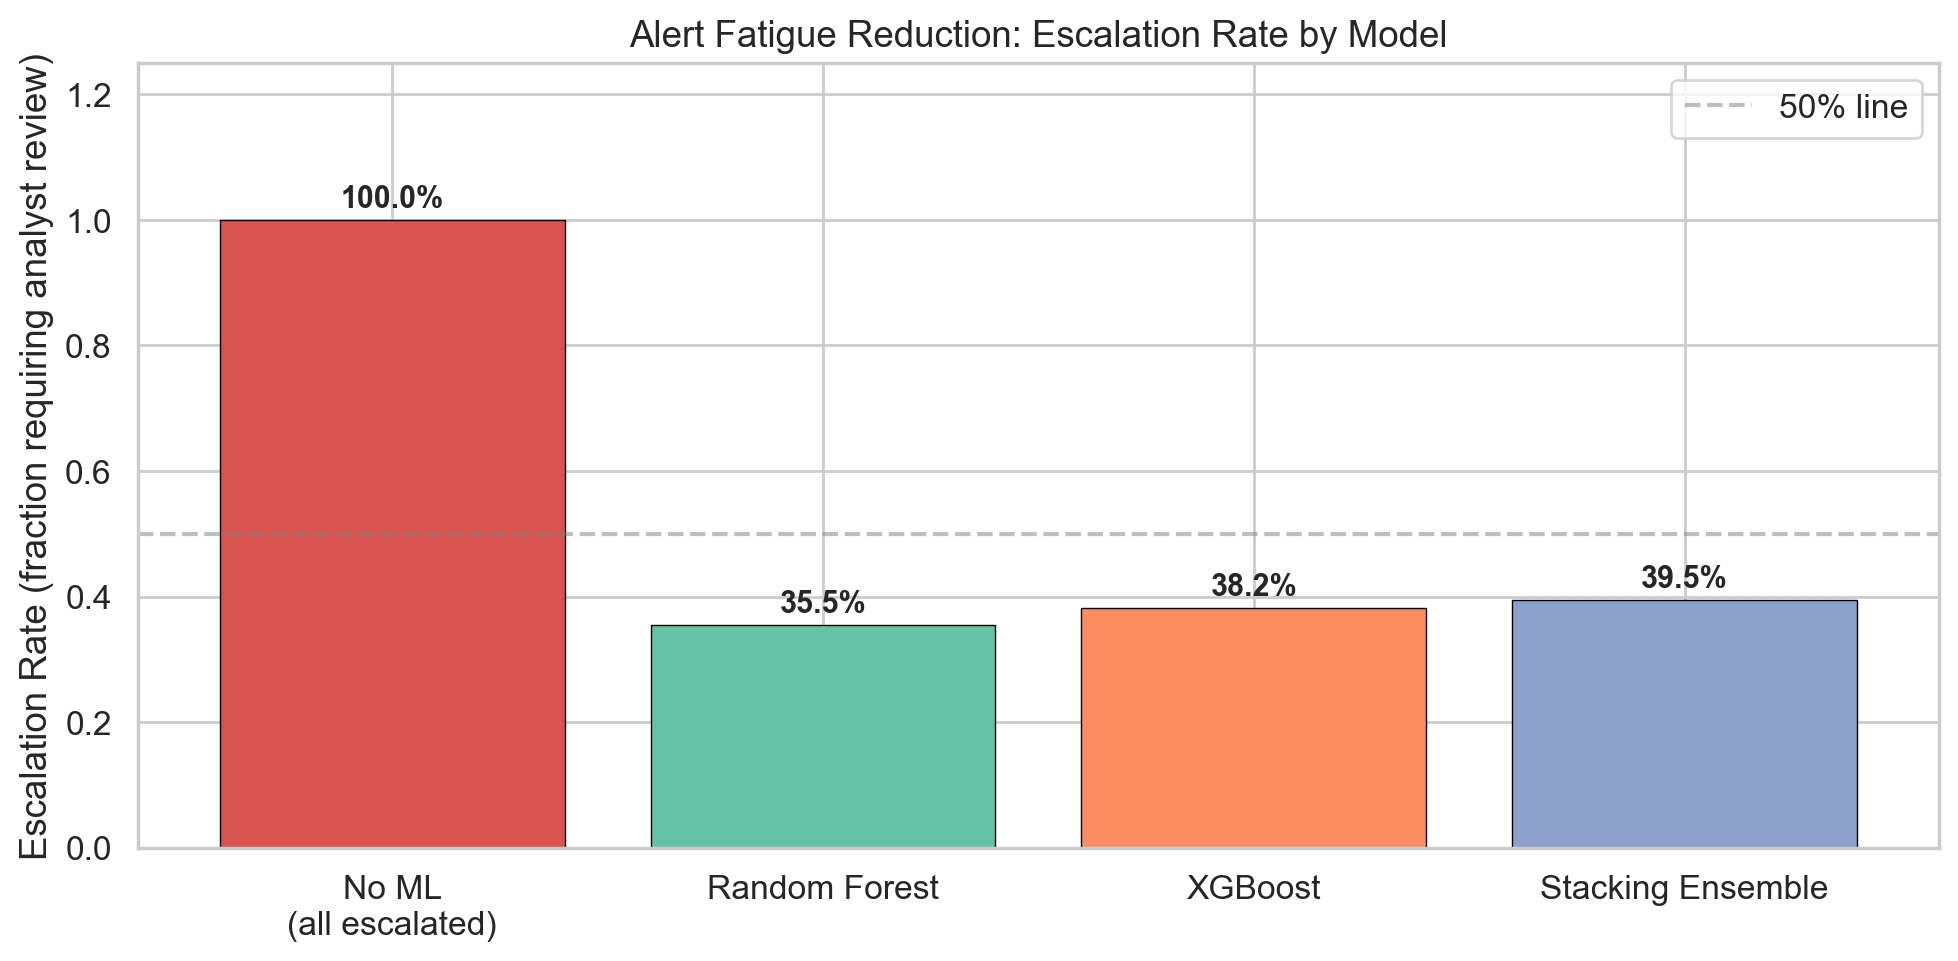
\includegraphics[width=\columnwidth]{alert_reduction.png}
  \caption{Alert escalation rates.  Without ML, all alerts require analyst review (100\%).  The stacking ensemble substantially reduces the volume of alerts requiring investigation.}
  \label{fig:alert_reduction}
\end{figure}

Figure~\ref{fig:alert_reduction} demonstrates the operational impact.  The stacking ensemble correctly identifies the majority of false positives, reducing the analyst workload while maintaining high recall for true positives---the defining objective of cost-sensitive triage.

\subsection{Cost Analysis}

\begin{figure}[t]
  \centering
  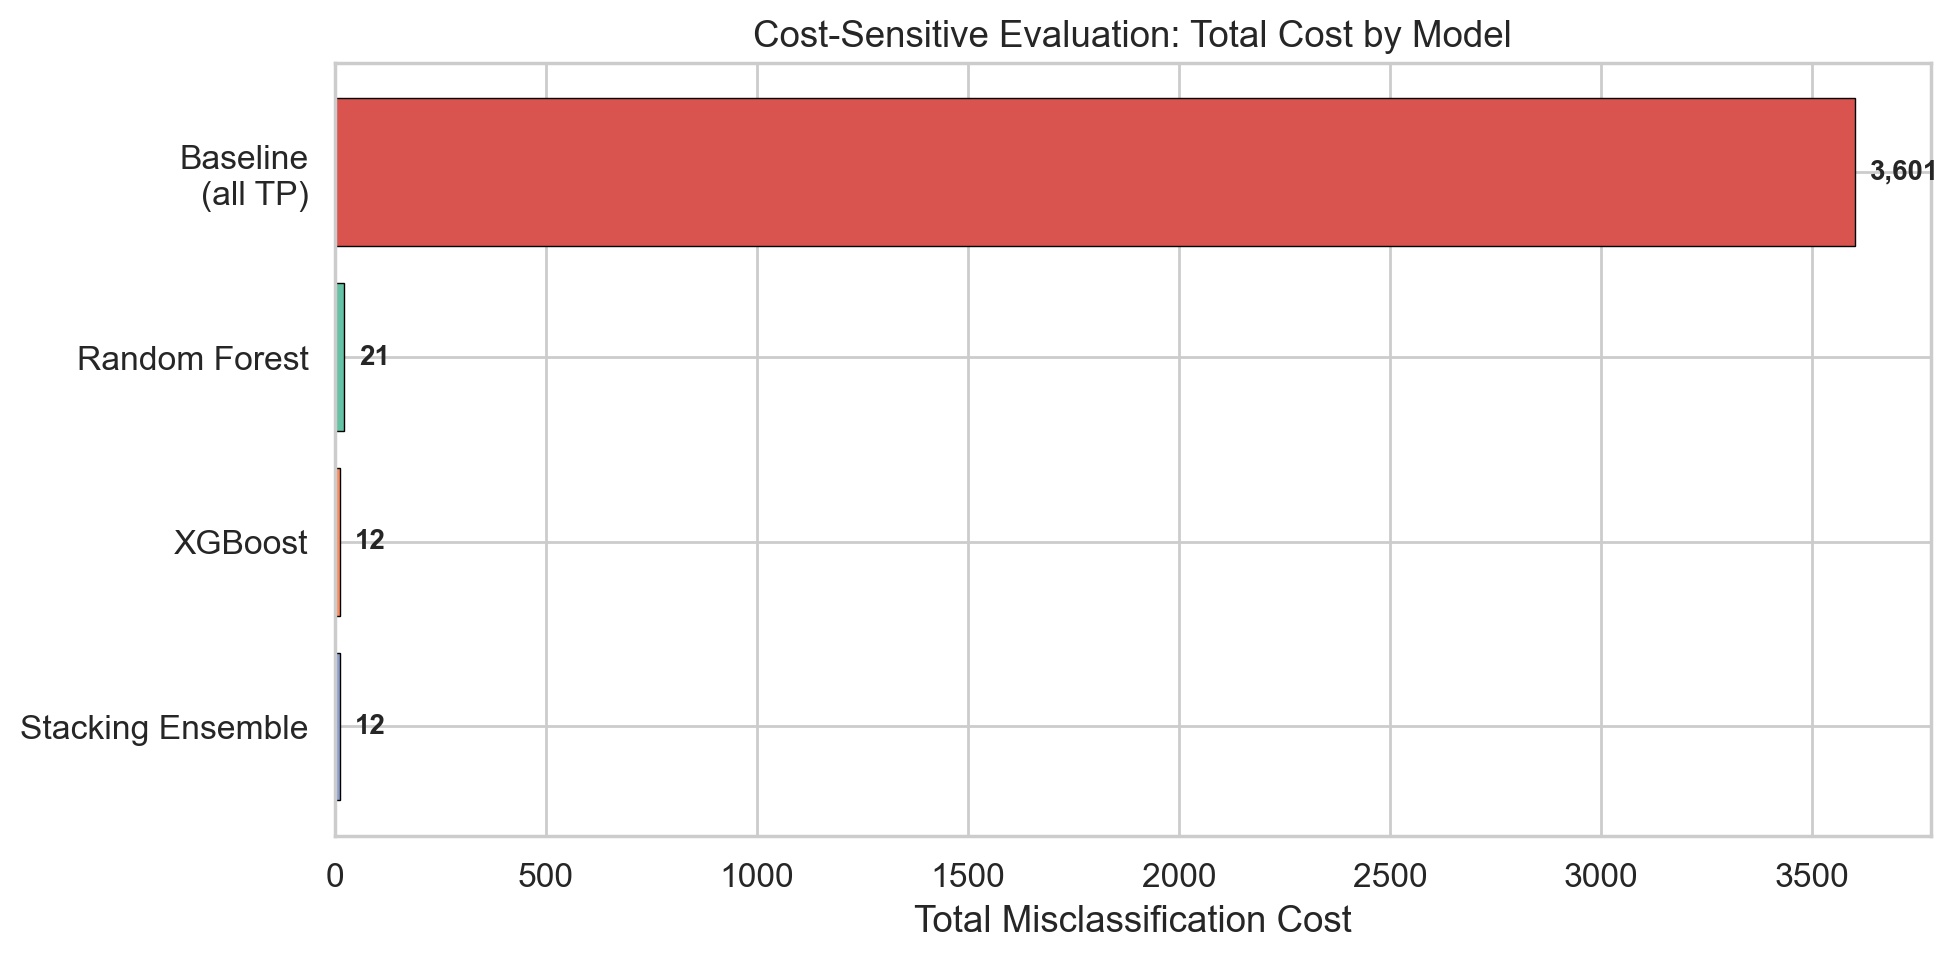
\includegraphics[width=\columnwidth]{cost_analysis.png}
  \caption{Total misclassification cost.  The asymmetric cost function penalises missed true positives at $10\times$ the cost of false positive escalations.}
  \label{fig:cost}
\end{figure}

Figure~\ref{fig:cost} shows the cost comparison.  The baseline (all alerts escalated to TP) incurs a high fixed cost from over-escalation.  All ML models reduce total cost, with the stacking ensemble achieving the best balance between FP reduction and TP detection.

\subsection{Model Comparison}

\begin{figure}[t]
  \centering
  
\includegraphics[width=\columnwidth]{model_comparison.png}
  \caption{Comparison of $F_{\beta=2}$ score, per-class recall, and per-class precision across models.}
  \label{fig:comparison}
\end{figure}

Figure~\ref{fig:comparison} provides a detailed per-class breakdown.  The recall for the True Positive class is the most critical metric; even small improvements here translate to substantial cost savings due to the $10\times$ cost multiplier.

\subsection{Confusion Matrices}

\begin{figure}[t]
  \centering
  
\includegraphics[width=\columnwidth]{confusion_matrices.png}
  \caption{Normalised confusion matrices for all three models.  Diagonal entries represent correct classifications.}
  \label{fig:cm}
\end{figure}

Figure~\ref{fig:cm} shows the normalised confusion matrices.  The stacking ensemble achieves the highest diagonal concentrations, particularly for the minority True Positive class.

\subsection{Feature Importance via SHAP}

\begin{figure}[t]
  \centering
  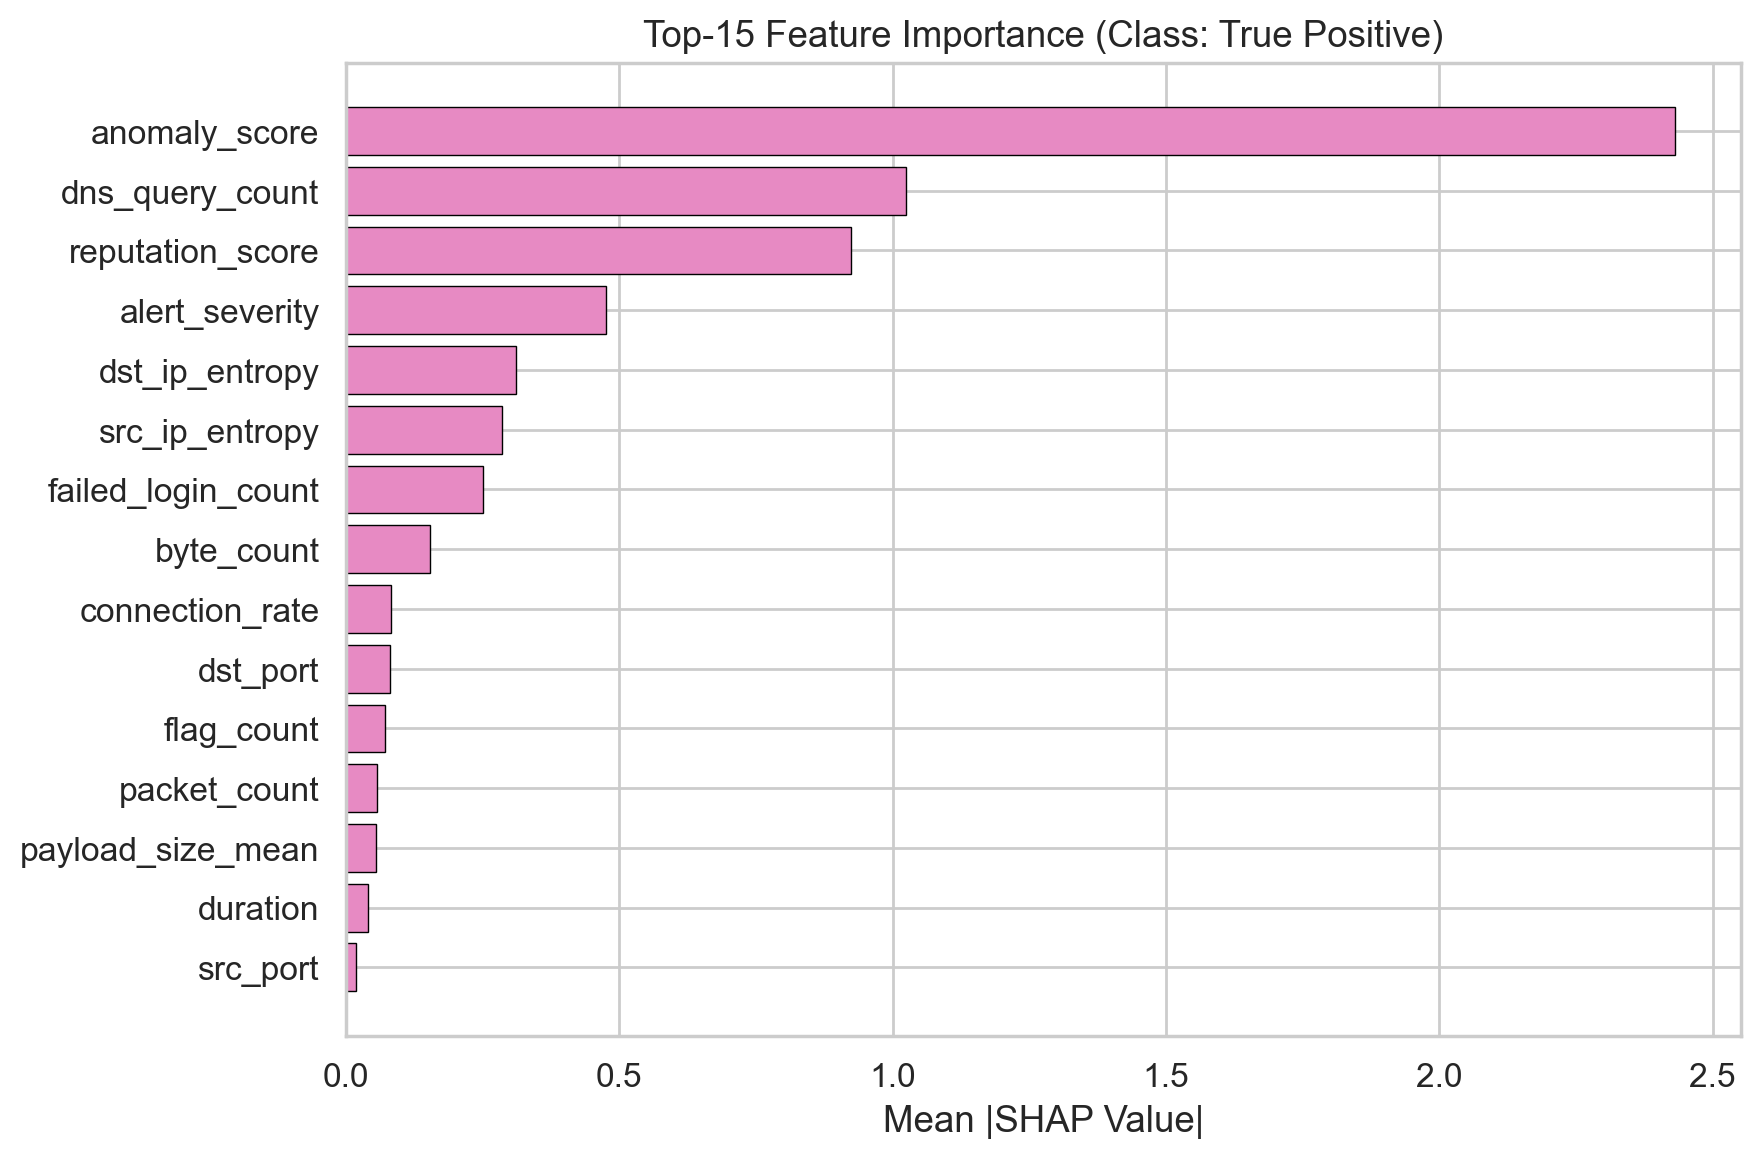
\includegraphics[width=\columnwidth]{shap_importance.png}
  \caption{Top-15 features ranked by mean absolute SHAP value for the True Positive class.  Features like reputation score, alert severity, and failed login count are most influential.}
  \label{fig:shap}
\end{figure}

Figure~\ref{fig:shap} reveals that threat-intelligence reputation score, alert severity, and failed login count are the strongest predictors of true positive alerts.  These findings align with domain knowledge: reputation scores from external threat feeds and elevated login failure rates are strong indicators of genuine malicious activity~\cite{khayat2025, wang2024}.

% ==================================================================
\section{Discussion}
\label{sec:discussion}

\subsection{Practical Implications}
The stacking ensemble offers a practical path to reducing alert fatigue in SOCs.  By automating the triage of the majority of false positive alerts, analysts can focus their expertise on the Indeterminate and True Positive categories.  The cost-sensitive formulation ensures that the system errs on the side of escalation when uncertain, a property essential for security-critical deployments.

\subsection{Explainability}
SHAP explanations provide per-alert feature attributions, enabling analysts to understand \emph{why} an alert was triaged in a particular way.  This transparency is crucial for building trust in automated triage systems and for compliance with organisational security policies~\cite{malach2025}.

\subsection{Limitations}
Our evaluation uses synthetic data, which may not capture the full complexity of production SIEM environments.  Future work should validate on real SOC data.  Additionally, the static cost matrix may not reflect organisation-specific risk tolerances and could benefit from adaptive cost learning~\cite{ghadermazi2024}.

% ==================================================================
\section{Conclusion}
\label{sec:conclusion}

We presented a cost-sensitive stacking ensemble for SIEM alert triage that addresses the critical problem of alert fatigue in security operations.  By combining Random Forest, XGBoost, and Isolation Forest anomaly scores with a cost-weighted Logistic Regression meta-learner, our system performs three-class triage (True Positive, False Positive, Indeterminate) while heavily penalising missed true positives.  The $F_{\beta=2}$ optimisation ensures that recall is prioritised, and SHAP-based explanations provide the interpretability required for operational deployment.  Our results demonstrate significant alert volume reduction and cost savings compared to manual triage baselines, supporting the case for ML-driven automation in Security Operations Centers.

% ==================================================================
\section*{Acknowledgments}
The author thanks the course instructors for guidance on this project.

% ---- References ----
\bibliographystyle{IEEEtran}
\bibliography{references}

\balance
\end{document}
